\section{Реализация пространственно\hyp{}антропометрической эргономической совместимости работника при разработке методов распознования, захвата и сопровождения движущихся объектов}

\subsection{Пространственно-антропометрическая эргономическая совместимость и ее сущность}
\emph{Эргономика} --- это научная дисциплина, комплексно изучающая человека в конкретных условиях его деятельности в современном производстве. Основной объект исследования эргономики --- \emph{система ``человек\hyp{}машина''}. Эргономические исследования и разработки заключаются в изучении человеко-машинных систем, а именно в исследовании характеристик человека, машины, окружающей среды, характера взаимодействия этих компонентов в конкретных условиях и организации производственной зоны, создании рабочих мест, машин, пультов управления, обеспечивающих максимальное удобство для человека, оптимальные условия взаимодействия с машиной и объектом управления.\cite{devisilov09}

На человека в процессе труда действует множество факторов: вид трудовой деятельности, ее тяжесть и напряженность, условия, в которой она осуществляется (вредный вещества, излучения, климатические условия, освещенность и т.д.), психофизиологические возможности человека (прежде всего антропометрические характеристика человека, скорость реакций на различные раздражители, особенности воприятия человеком цвета и т.д.). Для того чтобы человеко-машинная система функционировала эффективно и не приносила ушерба здоровью человека, необходимо прежде всего обеспечить совместимость характеристик машины и человека. Совместимость человека с машиной определяется его антропометрической, сенсомоторной, энергетической (биомеханической) и психофизиологической совместимостью.\cite{devisilov09}

Нас прежде всего интересует антропометрическая совместимость.

\emph{Антропометрическая совместимость} предполагает учет размеров тела человека, возможность обзора внешнего пространства, положения (позы) оператора в процессе работы при создании рабочего места.\cite{devisilov09}

Например, на рис.~\ref{access-zones} показаны антропометрические зоны досягаемости рук человека в положении стоя.

\begin{figure}
  \centering
  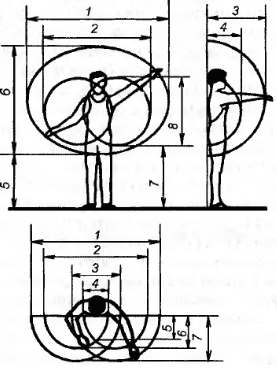
\includegraphics[width=0.4\textwidth]{images/devisilov-6-6}
  \caption{Зоны досягаемости рук человека в положении стоя в вертикальной и горизонтальной плоскостях: 1--8 --- номера зон\label{access-zones}}
\end{figure}

К антропометрическим характеристикам человека относятся статические характеристики --- размеры тела человека и его отдельных частей (головы, ног, рук, кистей, стоп, ширина плеч, таза и т.п.) и динамические характеристики -- возможные углы поворота отдельных частей тела, зоны досягаемости.\cite{devisilov09}

\begin{figure}
  \centering
  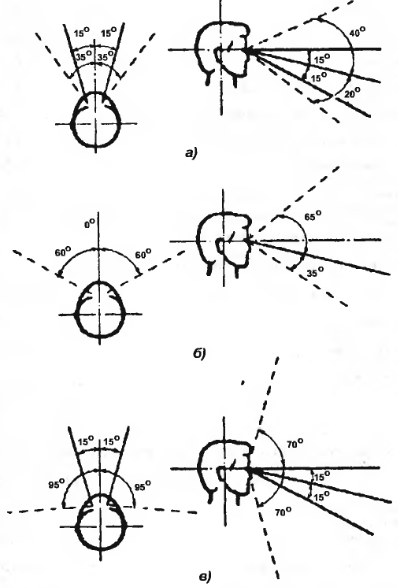
\includegraphics[width=0.75\textwidth]{images/devisilov-6-7}
  \caption{Информационные зоны визуального поля: а --- при повороте глаз; б --- при повороте головы; в --- при повороте головы и глаз; --- ---- оптимальные углы обзора; - - - --- максимальные углы обзора\label{visual-zones}}
\end{figure}

Информационные зоны визуального поля обзора человека представлены на рис.~\ref{visual-zones} и определяются полями зрения (поле ясного зрения, поле обзора и т.д.), размеры которых выражаются углами зрения.\cite{devisilov09}

\subsection{Трудовая функция работника, характеристика трудового процесса}
Характер и организация трудовой деятельности оказывают существенное влияние на изменение функционального состояния организма человека. Многообразные формы трудовой деятельности делятся на физический и умственный труд.\cite{belov09}

\emph{Физический труд} характеризуется нагрузкой на опорно\hyp{}двигательный аппарат и функциональные системы организма человека (сердечно-сосудистую, нервно-мышечную, дыхательную и др.), обеспечивающие его деятельность.\cite{belov09}

\emph{Умственный труд} объединяет работы, связанные с приемом и переработкой информации, требующей преимущественного напряжения сенсорного аппарата, внимания, памяти, а также активизации процессов мышления, эмоциональной сферы. Для данного вида труда характерна \emph{гипокинезия}, т.е. значительное снижение двигательной активности человека, приводящее к ухудшению реактивности организма и повышению эмоционального напряжения. Гипокинезия является одним из условий формирования сердечно-сосудистой патологии у лиц умственного труда. Длительная умственная нагрузка оказывает угнетающее влияние на психическую деятельность: ухудшаются функции внимания (объем, концентрация, переключение), памяти (кратковременной и долговременной), восприятия (появляется большое число ошибок).\cite{belov09}

Труд программиста является умственным (интеллектуальным). Более того он относится к наиболее сложной форме трудовой деятельности, требующей значительного объема памяти, напряжения, внимания, --- \emph{творческому труду}. Труд программистов приводит к значительному повышению нервно-эмоционального напряжения. При таком напряжении, связанном с умственной деятельностью, можно наблюдать тахикардию, повышение кровяного давления, увеличение легочной вентиляции и потребления кислорода, повышение температуры тела и другие изменения со стороны вегетативных функций человека.\cite{belov09}

Тяжесть и напряженность труда характеризуется степенью функциональнго напряжения организма. Оно может быть энергетическим, зависящим от мощности работы --- при физическом труде, и эмоциональным --- при умственным труде, когда имеет место информационная перегрузка.\cite{belov09}

Однообразие выполняемых операций приводит к определенному техническому состоянию человека, называемому \emph{монотомией}. Признаком монотомии является либо перегрузка одинаковой информацией, либо недостаток новой. Это накладывает отпечаток на функциональное состояние человека: он теряет интерес к выполняемой работе. Для него рабочее время как бы остановилось, и он с нетерпением джет окончания смены, его клонит ко сну. Монотонная работа снижает эффективность труда.\cite{belov09}

Физическая тяжесть труда программиста находится на минимальном уровне (программисту не надо поднимать грузы, делать частые наклоны и т.д.).
Чего нельзя сказать про напряженность труда.\cite{belov09}

\emph{Напряженность труда} характеризуется эмоциональной нагрузкой на организм при труде, требующем преимущественно интенсивной работы мозга по получению и переработке информации.\cite{belov09}

Программисту приходится работать с монитором более 4 ч. Деятельность программиста является творческой (эвристической) деятельностью, которая требует решения сложных задач при отсутствии очевидного алгоритма решения. Согласно \cite{belov09}, ее следует отнести к напряженному труду 2-й степени тяжести.

\subsection{Реализация требований пространственно\hyp{}антропометрической совместимости и проектирование рабочего места в соответствии с ними}
Организация рабочего места, конструкция органов контроля и управления должны учитывать антропометрические характеристики человека.\cite{devisilov09}

Оптимальное расположение и компоновка рабочего места, обеспечение удобной позы и свободы трудовых движений, использование оборудования, отвечающего требованиям эргономики и инженерной психологии, обеспечивают наиболее эффективный трудовой процесс, уменьшают утомляемость и предотвращают опасность возникновения профессиональных заболеваний.

Оптимальная поза человека в процессе трудовой деятельности обеспечивает высокую работоспособность и производительность труда. Неправильное положение тела на рабочем месте приводит к быстрому возникновению статической усталости, снижению качества и скорости выполняемой работы, а также к снижению реакции на опасности. Нормальной рабочей позой следует считать такую, при которой работнику не требуется наклоняться вперед больше, чем на \(10\dots15^{\circ}\); наклоны назад и в стороны нежелательны; основное требование к рабочей позе --- прямая осанка.

Работа в позе сидя более рациональна и менее утомительна, так как уменьшается высота центра тяжести над площадью опоры, повышается устойчивать тела, снижается напряжение мышц, уменьшается нагрузка на сердечно-сосудистую систему. В положении сидя обеспечивается возможность выполнять работу, требующую точность движения. Однако и в этом случае могут возникать застойные явления в органах таза, затруднение работы органов кровообращения и дыхания.

Смена позы приводит приводит к перераспределению нагрузки на группы мыщц, улучшению условий кровообращения, ограничивает монотонность. Поэтому, где это совместимо с технологией и условиями производства, необходимо предусматривать выполнение работы как стоя, так и сидя, с тем чтобы рабочие по своему усмотрению могли изменять положение тела.

\begin{figure}
  \centering
  \subfloat[][Зоны для выполнения ручных операций и размещения органов управления: 1 --- зона для размещения наиболее важных и очень часто используемых органов управления (оптимальная зона моторного поля); 2 --- зона для размещения часто используемых органов управления (зона легкой досягаемости моторного поля); 3 --- зона для размещения редко используемых органов управления (зона досягаемости моторного поля)]{\label{hand-operation-zones}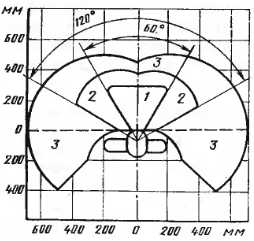
\includegraphics[width=0.4\textwidth]{images/devisilov-6-8}}
  \qquad
  \subfloat[][Зоны для выполнения ручных операций и размещения органов управления в вертикальной плоскости: 1 --- зона для размещения очень часто используемых и наиболее важных органов управления (оптимальная зона моторного поля); 2 --- зона для размещения часто используемых органов управления (зона легкой досягаемости моторного поля); 3 --- зона для размещения редко используемых органов управления (зона досягаемости моторного поля)]{\label{vertical-hand-operation-zones}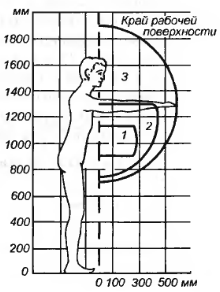
\includegraphics[width=0.4\textwidth]{images/devisilov-6-9}}
  \caption{}
\end{figure}

Пространство рабочего места, в котором осуществляются трудовые процессы, должно быть разделено на рабочие зоны. Зонирование рабочего места в горизонтальной и вертикальной плоскостях представлено на рис.~\ref{hand-operation-zones},~\ref{vertical-hand-operation-zones}. Рабочую зону, удобную для действия обеих рук, нужно обязательно совмещать с зоной визуального обзора.\cite{devisilov09}

Важное эргономическое значение имеет рабочая поза человека. Рабочая поза ``стоя'' требует больших энергетических затрат и приводит к быстрому утомлению. Рабочая поза ``сидя'' менее утомительно, и она более предпочтительно. Рабочая зона должна быть организована так, а органы управления должны быть так расположены, чтобы в рабочей позе проекция центра тяжести тела человека была расположена в пределах площади его опоры. В противном случае положение тела человека будет неустойчивым и потребует значительных мышечных усилий. Это может привести к заболеваниям опорно-двигательного аппарата (например, искривление позвоночника), быстрому утомлению, травме.\cite{devisilov09}

Составной частью рабочего места в положении ``сидя'' является рабочее кресло оператора. Кресло должно соответствовать антропометрическим данным человека. Основные геометрические параметры рабочих кресел стандартизованы. Целесообразно применять кресла с регулируемыми параметрами (высотой, углом, наклона спинки), чтобы приспособить их под антропометрические характеристики конкретного человека.\cite{devisilov09}

Устройства визуальной информации оператора в зависимости от частоты их использования также должны располагаться в соответствующих зонах визуального поля человека. При частом использовании приборы должны располагаться в пределах оптимальных углов обзора, при редком --- в пределах максимальных углов обзора.\cite{devisilov09}

\begin{figure}
  \centering
  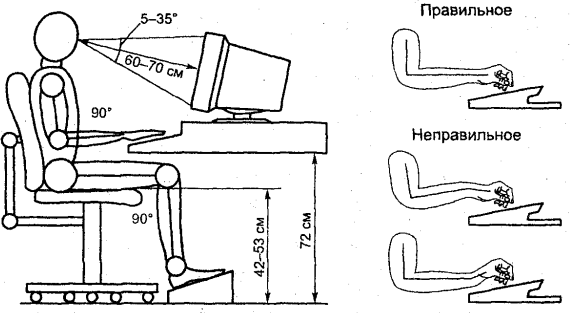
\includegraphics[width=0.9\textwidth]{images/mihnuk-3-14}
  \caption{Правильная позиция оператора и положение его рук при работе на клавиатуре\label{operator-position}}
\end{figure}

Уровень глаз при вертикальном расположенном экране видеодисплея должен приходиться на центр или \(^2/_3\) высоты экрана. Линия взора должна быть перпендикулярна к центру экрана. При работе на клавиатуре необходимо соблюдать правильное положение рук оператора (рис~\ref{operator-position}).\cite{mihnuk07}

Расположение рабочих мест для пользователей видеодисплеев и ПЭВМ в подвальных помещениях не допускается.\cite{mihnuk07}

Площадь на одно рабочее место с видеодисплеем и ПЭВМ должна составлять не менее \(6,0 \text{м}^2\), а объем --- не менее \(20,0 \text{м}^3\).\cite{mihnuk07}

При размещении рабочих мест расстояние между рабочими столами должно быть не менее \(2,0 \text{м}\), а расстояние между боковыми поверхностями видеомониторов --- не менее \(1,2 \text{м}\). Рабочие места сотрудников, выполняющих творческую работу и требующей значительного умственного напряжения или высокой концентрации внимания, рекомендуется изолироваться друг от друга перегородками высотой от \(1,5 \text{м}\).\cite{mihnuk07}

Рабочие столы следует размещать таким образом, чтобы мониторы были ориентированы боковой стороной к световым проемам, чтобы естественный свет падал преимущественно слева.
\newpage
